\section{Work Packages}
\label{sec:work-packages}

Figure~\ref{fig:wps} shows the work package breakdown for SECT-AIR, including their interrelationships. 

\begin{figure}[htbp]
\centerline{\scalebox{0.7}{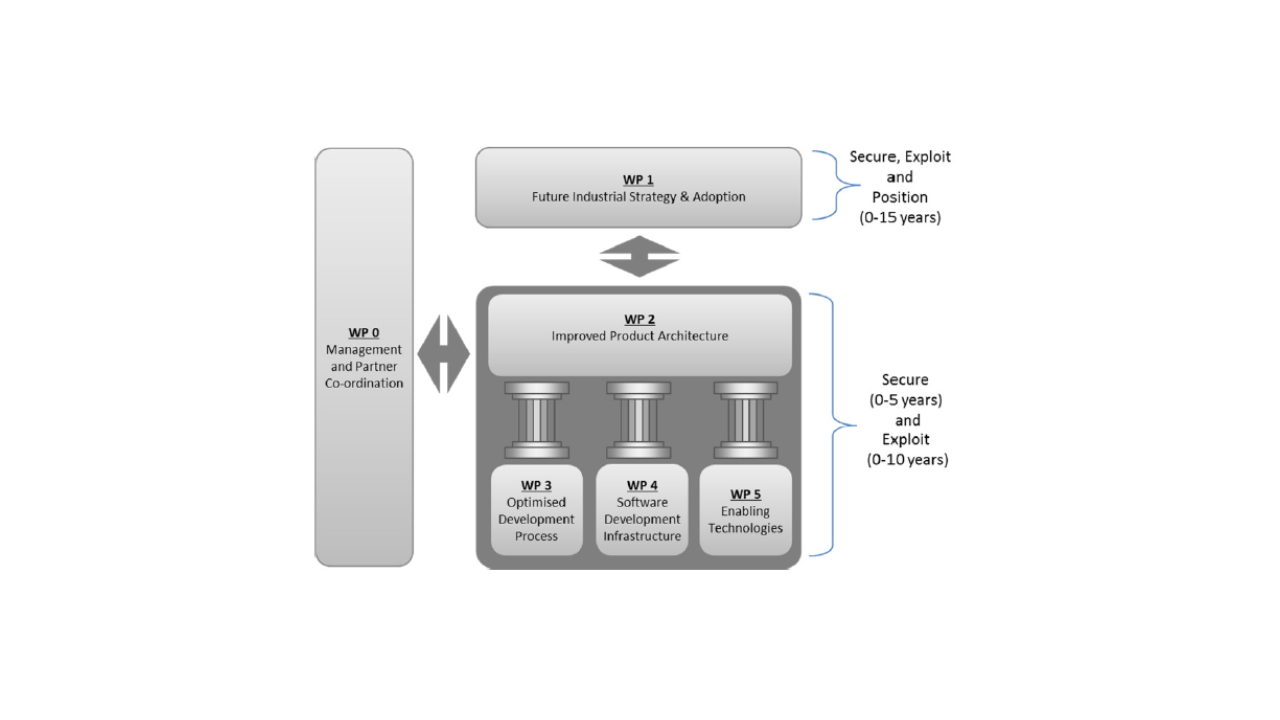
\includegraphics{work-packages.png}}}
\caption{Work package structure for SECT-AIR}
\label{fig:wps}
\end{figure}

Work Package (WP1) focuses
on industry strategy and adoption of SECT-AIR deliverables: it includes baselining activities to measure current state of practice in aerospace software engineering, and will
support experiments designed to demonstrate potential improvements. It also aims to create a long-term industry strategy (for 10-15 years)
that will ensure significant industry and academic alignment. It will be responsible for coordinating usable case study material for research in other work
packages.

WP2 focuses on developing a common open and modular product architecture for aerospace software engineering, which will in turn enhance the product
supply chain. It will also investigate the use of partitioning in aerospace products to reduce the amount of safety-critical functionality within embedded products.
It will deliver demonstrators of open architectures at high technical readiness levels. The open architecture will be evaluated via demonstrator case studies that
will be identified in WP1.

WP3 investigates software development processes. It is particularly targeting the application and evaluation of model-based techniques for requirements
specification, to ensure composability and reuse of requirements: the view is that across a number of aerospace projects (requiring certification) there is a significant opportunity to reuse requirements -- especially if they can be captured in a standard and tool-supported modelling language. As well, WP3 will investigate traceability and will build a toolchain to support end-to-end
traceability from requriements models through to documentation and code. WP3 will in parallel trial the application of formal specification techniques used in
synergy with model-based techniques to support richer analysis of requirements. The techniques that are developed will be applied to case studies that
focus on novel interactive interfaces, e.g., for cockpit display systems. Such systems benefit from the development of rapid prototypes (even for critical
systems) and thus make a challenging case study for model-based and formal methods, especially given that minimising the cost and time to change,
for example, display formats, is an industry-wide issue in aerospace.

WP4 focuses on software development infrastructure for aerospace software engineering. It will endeavour to set a UK strategy for software development
infrastructure improvements, and  develop tool support to provide integration to various model-based languages used by industry, e.g., SysML, UML and
various UML profiles such as MARTE. It will also aim to reduce the overhead for code-level verification and for generating qualification and assurance data.
We discuss WP4 in more detail in the next subsection.

WP5, Enabling Technologies, aims to deliver a roadmap and demonstrator for next-generation high-performance obsolescence protected platforms. In particular
it will aim to reduce the effort and costs for producing high-integrity firmware, such as system-on-chip and many-core processors. It will also work with certification
authorities to ensure that the best practice that is developed will lead to systems that can achieve certification. A particular technique that will be investigated will
be modular component-based development.

\subsection{Model-based development}
WP4 broadly focuses on software development infrastructure -- i.e., producing a common platform (largely via reuse and agreement on standards) -- for aerospace
software engineering. The vision is to exploit model-based development techniques as a means to increase productivity and to automate the error-prone, repetitive
and tedious tasks of engineers. There are three components to achieving this vision:
\begin{itemize}
\item Exploiting model-based languages, including general-purpose languages (and tools) as well as techniques for building domain-specific languages for specific problems. 
There is broad agreement on the use of (profiles of) UML and SysML throughout SECT-AIR, and the project partners have predominantly agreed on the use of Eclipse
Papyrus for many of their modelling needs within the project. A key requirement is to support efficient and effective development of UML profiles for individual partners,
including those partners who have limited-to-no experience of building profiles. Thus, one objective of WP4 is to investigate new and efficient ways of \textit{generating}
profiles for UML and SysML, maximising reuse (e.g., when two or more profiles share features).

\item Providing support for efficient and effective model transformations. Many partners in SECT-AIR need transformations to allow them to use new modelling
technology such as Eclipse Papyrus in combination with legacy modelling technology, such as Artisan PTC Modeller. A particular objective of this work package is to
ensure that any enabling model transformation technology is efficient, even when applied to large and complicated models. As such, WP4 is investigating 
\textit{incremental} model transformations, where small changes to the source models mean that only small parts of the transformations need to be executed
again. One of the techniques that will be considered for use is property traces, which have been used to support incremental code generation \cite{OgunyomiRK15}.


\item Generating text and documentation. A particular use case for generation of text is producing
template \textit{assurance cases} from engineering artefacts (e.g., UML design models). Template assurance cases provide the structure and outline of an assurance
argument that -- after refinement and instantiation -- will be delivered to a certifying authority along with evidence (e.g., test data, traceability data). Such arguments are
and evidence are critical in attempting to convince the certifying authority that a system is acceptably safe to deploy in its environment. Producing assurance cases is
generally carried out manually and is an expensive process. Recertifying a system where requirements have changed is also a very expensive process. Hence, there is strong
benefit from  using model-to-text transformation to at least partly automate the process of producing assurance cases. SECT-AIR will investigate preliminary work on using weaving models \cite{HawkinsHKPK15} to underpin the process of generating template assurance cases from engineering artefacts supplied by industry partners.
\end{itemize}

Case studies from industry partners focusing on security and safety-critical systems development are being identified to help demonstrate the effectiveness
of the techniques developed in this work package.



